\documentclass[tikz,border=8pt]{standalone}
% Shared look for every TikZ diagram. Load with % Shared look for every TikZ diagram. Load with % Shared look for every TikZ diagram. Load with \input{../../tools/tikz-style.tex}
\usepackage[T1]{fontenc}
\usepackage{lmodern}
\renewcommand{\sfdefault}{lmr}  % diagrams use the same serif as the text
\usetikzlibrary{arrows.meta, positioning, shapes.geometric, calc, fit, backgrounds}
\definecolor{cblue}{HTML}{4C78A8}
\definecolor{corange}{HTML}{F58518}
\definecolor{cgreen}{HTML}{54A24B}
\definecolor{cred}{HTML}{E45756}
\definecolor{cpurple}{HTML}{B279A2}
\definecolor{cgrey}{HTML}{6B6B6B}
\tikzset{
  every picture/.style={font=\sffamily, line width=1.2pt},
  box/.style={draw=#1, fill=#1!12, rounded corners=4pt, align=center, inner sep=7pt, minimum height=1.1cm},
  box/.default=cgrey,
  arrow/.style={-{Stealth[length=3mm]}, draw=cgrey, line width=1.4pt},
  title/.style={font=\sffamily\bfseries\Large},
  note/.style={font=\sffamily\small, text=cgrey, align=center},
}
\AtBeginDocument{\hyphenpenalty=10000 \exhyphenpenalty=10000}

\usepackage[T1]{fontenc}
\usepackage{lmodern}
\renewcommand{\sfdefault}{lmr}  % diagrams use the same serif as the text
\usetikzlibrary{arrows.meta, positioning, shapes.geometric, calc, fit, backgrounds}
\definecolor{cblue}{HTML}{4C78A8}
\definecolor{corange}{HTML}{F58518}
\definecolor{cgreen}{HTML}{54A24B}
\definecolor{cred}{HTML}{E45756}
\definecolor{cpurple}{HTML}{B279A2}
\definecolor{cgrey}{HTML}{6B6B6B}
\tikzset{
  every picture/.style={font=\sffamily, line width=1.2pt},
  box/.style={draw=#1, fill=#1!12, rounded corners=4pt, align=center, inner sep=7pt, minimum height=1.1cm},
  box/.default=cgrey,
  arrow/.style={-{Stealth[length=3mm]}, draw=cgrey, line width=1.4pt},
  title/.style={font=\sffamily\bfseries\Large},
  note/.style={font=\sffamily\small, text=cgrey, align=center},
}
\AtBeginDocument{\hyphenpenalty=10000 \exhyphenpenalty=10000}

\usepackage[T1]{fontenc}
\usepackage{lmodern}
\renewcommand{\sfdefault}{lmr}  % diagrams use the same serif as the text
\usetikzlibrary{arrows.meta, positioning, shapes.geometric, calc, fit, backgrounds}
\definecolor{cblue}{HTML}{4C78A8}
\definecolor{corange}{HTML}{F58518}
\definecolor{cgreen}{HTML}{54A24B}
\definecolor{cred}{HTML}{E45756}
\definecolor{cpurple}{HTML}{B279A2}
\definecolor{cgrey}{HTML}{6B6B6B}
\tikzset{
  every picture/.style={font=\sffamily, line width=1.2pt},
  box/.style={draw=#1, fill=#1!12, rounded corners=4pt, align=center, inner sep=7pt, minimum height=1.1cm},
  box/.default=cgrey,
  arrow/.style={-{Stealth[length=3mm]}, draw=cgrey, line width=1.4pt},
  title/.style={font=\sffamily\bfseries\Large},
  note/.style={font=\sffamily\small, text=cgrey, align=center},
}
\AtBeginDocument{\hyphenpenalty=10000 \exhyphenpenalty=10000}

\begin{document}
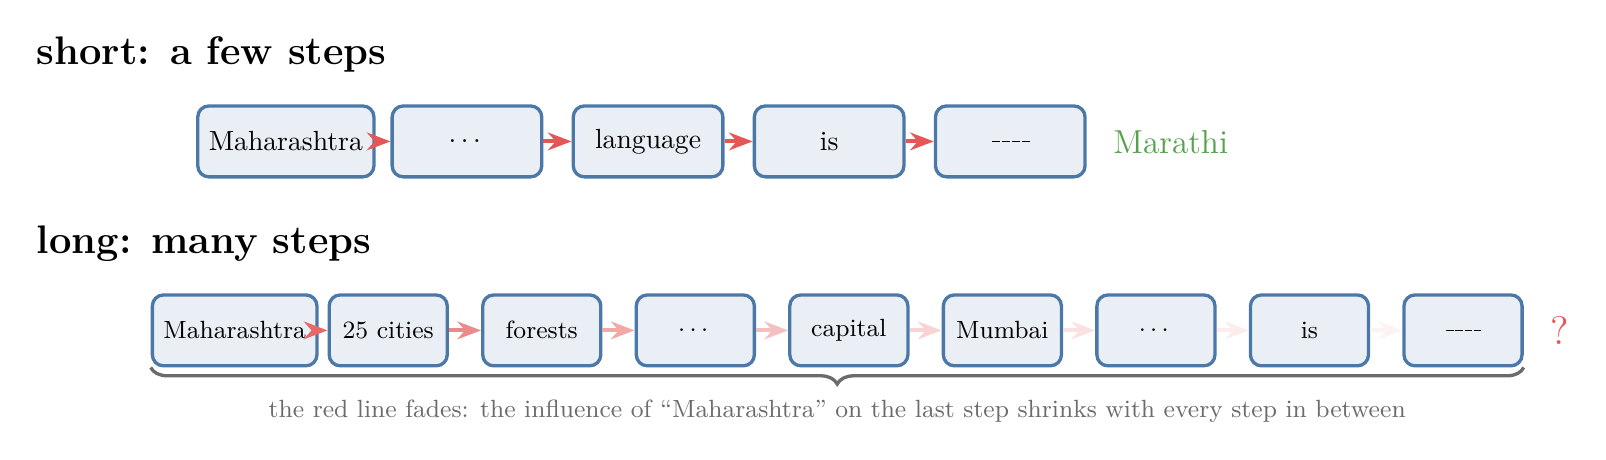
\begin{tikzpicture}[w/.style={box=cblue, minimum width=1.9cm, minimum height=0.9cm, inner sep=4pt}]
  % short sentence
  \node[title, anchor=west] at (-1,2.3) {short: a few steps};
  \foreach \word [count=\i] in {Maharashtra, \dots, language, is, \_\_\_\_}
    \node[w] (s\i) at (2.3*\i,1.2) {\word};
  \foreach \i [evaluate=\i as \j using int(\i+1)] in {1,...,4} \draw[arrow, draw=cred] (s\i) -- (s\j);
  \node[note, anchor=west, text=cgreen, font=\sffamily\large] at ([xshift=0.2cm]s5.east) {Marathi};
  % long sentence
  \node[title, anchor=west] at (-1,-0.1) {long: many steps};
  \foreach \word/\op [count=\i] in {Maharashtra/100, 25 cities/75, forests/55, \dots/38, capital/25, Mumbai/16, \dots/10, is/6, \_\_\_\_/4}
    \node[w, minimum width=1.5cm, font=\sffamily\small] (l\i) at (1.95*\i-0.3,-1.2) {\word};
  \foreach \i/\op [evaluate=\i as \j using int(\i+1)] in {1/90, 2/70, 3/52, 4/38, 5/26, 6/17, 7/11, 8/7}
    \draw[arrow, draw=cred!\op] (l\i) -- (l\j);
  \node[note, anchor=west, text=cred, font=\sffamily\Large] at ([xshift=0.2cm]l9.east) {?};
  \draw[decorate, decoration={brace, mirror, amplitude=6pt}, cgrey] (l1.south west) -- node[note, below=8pt] {the red line fades: the influence of ``Maharashtra'' on the last step shrinks with every step in between} (l9.south east);
\end{tikzpicture}
\end{document}
